\chapter{Conclusiones y recomendaciones}

Después de realizar este informe la principal conclusión a la que se puede llegar es que si bien moodle es una base idónea para desarrollar el sistema de gestión de la docencia online de la Universidad de Granada pensamos que se deberían realizar una serie de cambios y ajustes para adecuarlo a las necesidades propias de la Universidad.

\bigskip
Quiero hacer hincapié en el gran esfuerzo realizado por los profesionales del CEVUG y no quiero que este análisis se entienda como una crítica hacia su excelente trabajo. Con mi experiencia como desarrollador web puedo afirmar que no es fácil tener en cuenta los miles de detalles requeridos para personalizar, adaptar y optimizar una plataforma y mas cuando se trabaja a contrarreloj solucionando problemas lo que en muchos casos no permite mas que hacer un ajuste "temporal" que perdura en el tiempo indefinidamente. Por ello este informe, aunque dirigido a ellos como ayuda para optimizar la plataforma quizá debería servirles para hacer ver a sus superiores que algo tan importante como la plataforma web de apoyo a la docencia debería tener mas medios.

\bigskip
Sólo como nota, para gestionar su cuenta de twitter la policía nacional de España cuenta con un equipo de 8 personas a tiempo completo. Prado, que evidentemente es mas complejo y requiere muchísimo más trabajo actualmente no cuenta con ningún desarrollador y las tres personas a cargo solo realizan tareas de administración de la plataforma.

\bigskip

La filosofía del software libre no se limita a distribuir software de forma gratuita, la idea es que al estar disponible el código fuente la gente pueda participar en el proyecto realizando modificaciones y mejoras. Si por el contrario nos limitamos a hacer uso del software sin aportar nada a la comunidad de desarrolladores estamos haciendo un flaco favor y además al venir esto de una institución donde se imparte conocimiento el efecto es aun mayor. Por lo pronto se debería mostrar de forma claro tanto que se está usando moodle como un enlace a su sitio original así como su licencia, cosa a la que de hecho obliga la licencia GPLv3 bajo la que está liberado moodle.

\bigskip
También hay que tener en cuenta que ante cualquier cambio los usuarios siempre oponen resistencia sea el cambio para mejor o para peor Esto siempre hay que tenerlo en cuenta a la hora de interpretar las críticas hacia el sistema.

\bigskip
Es evidente que en el estado actual y con los recursos existentes no se puede competir con otras plataformas con muchos años a sus espaldas como puede ser SWAD, por eso quizá no sea mala idea en lugar de intentar acercarse a lo ya existente plantearse otro objetivo como puede ser la simplicidad. Como ya hemos visto la mayor parte de los usuarios necesitan un pequeño porcentaje de funciones. ¿Por qué no ocultar el resto? Imaginemos Prado como una plataforma basada en cuatro pilares fundamentales: Documentos, Tareas, Calificaciones y Mensajería. Si ocultamos el resto de opciones tenemos un sistema bastante más simple que el actual y seguramente sería suficiente para el 95\% de los usuarios.

\bigskip
Una vez realizada esta simplificación ya se podrían empezar a agregar funciones en base a su necesidad, pero sin olvidarnos de la máxima de la plataforma, que sería la simpleza. 

\bigskip
Javier Krahe decía en una canción: \textit{'...en Villatripas de Abajo se suple con desparpajo por parte del vecindario la falta de monetario...'}. Y partiendo de esa idea se podría resolver la falta de recursos del CEVUG creando en la ETSIIT una asignatura sobre programación de plataformas tipo moodle y que los propios alumnos fueran mejorando la plataforma. 

\newpage
En cuanto a futuras mejoras de la plataforma Prado2 vamos a clasificarlas las mejoras sugeridas en carácter urgente, recomendado y opcional:

\section{Mejoras de carácter urgente}

\begin{itemize}
	\item Configurar Prado para que sirva todo el contenido exclusivamente vía HTTPS, para esto solo hay que activar la opción en la configuración de moodle y se conseguiría solucionar el problema de seguridad del secuestro de sesiones.

	\item Actualizar la versión de moodle, ya que en un entorno web en constante evolución no es admisible quedarse en versiones anticuadas que a la larga pueden acarrear serios problemas de seguridad y compatibilidad.

	\item Dejar todos los menús laterales visibles, ya que la implementación actual del template no respeta los anteriormente abiertos y crea mucha confusión al usuario al no saber donde se está
\begin{lstlisting}
# regla css para mostrar desplegados todos los paneles
.block {
	display: block;
}
\end{lstlisting}

	\item Ocultar las vistas no necesarias como "Todos los cursos".
	\item Ocultar para los alumnos el menú lateral derecho de "Problemas"
	\item Mostrar el mensaje de información a la hora de editar un curso para saber que se pueden arrastrar ficheros directamente.
	\item Ocultar la barra superior de idioma y poner en su lugar un enlace en el pie de la página.
	\item Ocultar el menú superior o poner unas opciones mas útiles.
	\item Simplificar el interfaz del sistema de mensajería.
	\item Ocultar el banner central, o mostrarlo solamente a los usuarios no identificados.
	\item Utilizar una redirección 301 en \url{http://prado.ugr.es/index.html} configurando el archivo \texttt{.htaccess} ya que esto reduciría las peticiones al servidor.
\begin{lstlisting}
# redirección 301
Redirect 301  /index.html https://prado.ugr.es/moodle/index.php
\end{lstlisting}
	
	\item Revisar que en script de sincronización entre la base de datos institucional y prado todo esté funcionando con UTF-8 para no encontrar problemas con los nombres de los alumnos.


	\item Bloquear en el fichero \texttt{.htaccess} el acceso a ficheros \texttt{README} y \texttt{CHANGELOG} y otros ficheros auxiliares como medida de seguridad.
\begin{lstlisting}
# ocultar archivos .txt, readmes, etc..
<IfModule mod_rewrite.c>
    RewriteCond %{REQUEST_URI} !/robots\.txt$ [nocase]
    RewriteRule \.txt$  -  [forbidden,last]
    RewriteRule \.xml$  -  [forbidden,last]
    RewriteRule \.md$  -  [forbidden,last]
</IfModule>
\end{lstlisting}	
	
	
\end{itemize}


\section{Mejoras de carácter recomendado}

\begin{itemize}
	\item Desactivar las insignias.
\begin{figure}[H]
\centering
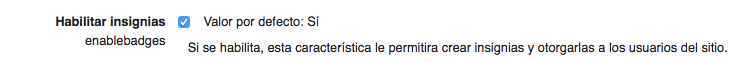
\includegraphics[width=1.0\textwidth]{../screenshots/desactivar_insignias}
\caption{Desactivar insignias}
\end{figure}	
	\item Instalar una plantilla con un diseño mas sencillo.
	\item Desactivar las actividades menos utilizadas o al menos no mostrarlas todas a la hora de crear una nueva actividad.
	\item Instalar el plugin material download moodle plugin\cite{moodleplugin} para permitir descargar todos los contenidos de un curso de golpe.
	\item Desactivar los blogs de la asignatura.
\begin{figure}[H]
\centering
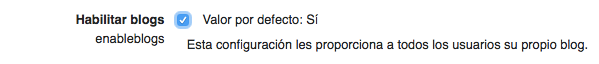
\includegraphics[width=1.0\textwidth]{../screenshots/desactivar_blogs}
\caption{Desactivar blogs}
\end{figure}	
\end{itemize}

\section{Mejoras de carácter opcional}
\begin{itemize}
	\item Activar los servicios web XML de moodle y utilizar el código fuente de las aplicación Android e iOS propias de moodle para desarrollar unas versiones propias que hagan uso del IDP del CSIRC.
\begin{figure}[H]
\centering
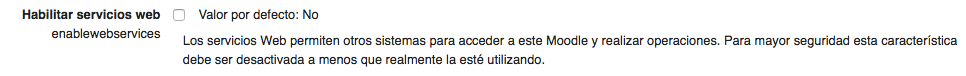
\includegraphics[width=1.0\textwidth]{../screenshots/habilitar_serviciosweb}
\caption{Habilitar servicios web}
\end{figure}

	\item Unificar las vistas de curso para verlo todo de un vistazo.
	
\end{itemize}

\section{Temporización final}

En la figura \ref{fig:temporizacion2} podemos ver un diagrama con los tiempos empleados para el desarrollo de este proyecto. 

\begin{figure}[H]
\centering
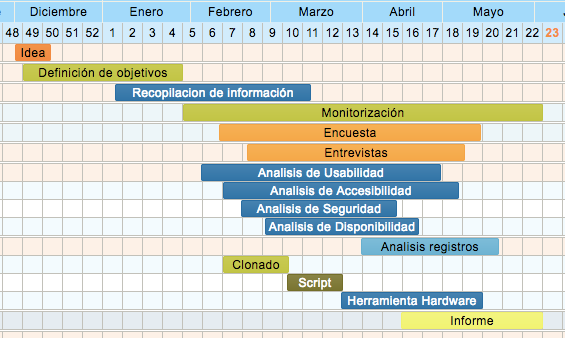
\includegraphics[width=0.8\textwidth]{../screenshots/temporizacion2}
\caption{Diagrama de Gantt con los tiempos invertidos en el proyecto}
\label{fig:temporizacion2}
\end{figure}

Los hitos más importantes en el desarrollo de este proyecto han sido los siguientes:

\begin{itemize}
	\item Septiembre 2014 - Primera contacto con Prado2

    \item Octubre 2016. Empieza a gestarse la idea de realizar un TFG sobre Prado2.
    
    \item Noviembre 2016. Se sientan las bases del proyecto. Se empiezan a recoger sugerencias de los usuarios.
    
    \item Enero 2016. Comenzamos a monitorizar la disponibilidad plataforma.
    
    \item Febrero 2016. Se lanza la encuesta a los usuarios de Prado.
    
    \item Marzo 2017 - Contactamos con los administradores de Prado2 para ver puntos de actuación en común y ver su punto de vista sobre la plataforma.
    
    \item Abril 2017. Se comienza a redactar la memoria.

    \item Mayo 2017. El CEVUG nos proporciona los logs de Prado.
    
    \item Junio 2017. Defensa final del proyecto

\end{itemize}
